\documentclass[aps,showpacs,twocolumn,floats,prd,superscriptaddress,nofootinbib]{revtex4-1} 
\usepackage{graphicx,amsmath,amssymb,amstext}
\usepackage{amssymb,amsbsy,amsfonts,amsthm,color}
\usepackage{epsfig}
%\usepackage{showkeys}
\usepackage{graphicx}
\usepackage{subfigure}
\usepackage{sidecap}
\usepackage{floatrow}
\graphicspath{{Figures/}}

\begin{document}

\title{On the limitations of using quantum mechanics in a fixed background of a Schwarzschild black hole}

\author{Daniel Baker}
\email{dbaker@cita.utoronto.ca}
\affiliation{Canadian Institute of Theoretical Astrophysics, 60 St George St, Toronto, ON M5S 3H8, Canada.}
\affiliation{University of Toronto, Department of Physics, 60 St George St, Toronto, ON M5S 3H8, Canada.}

\author{Darsh Kodwani}
\email{dkodwani@physics.utoronto.ca}
\affiliation{Canadian Institute of Theoretical Astrophysics, 60 St George St, Toronto, ON M5S 3H8, Canada.}
\affiliation{University of Toronto, Department of Physics, 60 St George St, Toronto, ON M5S 3H8, Canada.}

\author{Ue-Li Pen}
\email{pen@cita.utoronto.ca}
\affiliation{Canadian Institute of Theoretical Astrophysics, 60 St George St, Toronto, ON M5S 3H8, Canada.}
\affiliation{Canadian Institute for Advanced Research, CIFAR program in Gravitation and Cosmology.}
\affiliation{Dunlap Institute for Astronomy \& Astrophysics, University of Toronto, AB 120-50 St. George Street, Toronto, ON M5S 3H4, Canada.}
\affiliation{Perimeter Institute of Theoretical Physics, 31 Caroline Street North, Waterloo, ON N2L 2Y5, Canada.}

\author{I-Sheng Yang}

\email{isheng.yang@gmail.com}
\affiliation{Canadian Institute of Theoretical Astrophysics, 60 St George St, Toronto, ON M5S 3H8, Canada.}
\affiliation{Perimeter Institute of Theoretical Physics, 31 Caroline Street North, Waterloo, ON N2L 2Y5, Canada.}

\begin{abstract}
Abstract
\end{abstract}

\maketitle


\onecolumngrid

\section{Introduction}

%Whenever we describe a quantum system, we assume that the system we are describing and the environment around it are separate things. In particular we assume the environment can be described classically and the system we are describing behaves quantum mechanically. There are points where this assumption breaks down and we can see a clear example of this in terms of the interference pattern of a double slit experiment(DESCRIBE THE SITUATION INVOLVING THE DOUBLE SPLIT EXPERIMENT HERE). In this paper we analyse when this description of quantum mechanics in a classical background breaks down in the presence of a BH.

\section{Calculation}

\subsection{Proper time}

\subsubsection{Background spacetime}


First we consider the motion of Hawking photons coming from a Schwarzschild metric of the form

\begin{equation}
	ds^2 = - \left( 1 - \frac{2M}{r} \right) dt^2 + \left( 1 - \frac{2M}{r} \right)^{-1} dr^2 + r^2 d \Omega_2^2.
\end{equation}

Consider two Hawking photons coming from a fixed distance, $r_{e}$, just above a Schwarzschild black hole separated by a coordinate time interval $\bar{\delta t}_A$ and a corresponding proper time $\bar{\delta \tau}_A$ as shown in figure \ref{fig:1}. The two photons propagate through to the observer at $r_0$ following geodesics. We could potentially solve for the geodesics of the photons to find out the coordinate time of arrival of each photon, however in the absence of additional gravitational fields the coordinate time interval between the photons will not change\footnote{This will prove to be extremely helpful when we look at the calculation in the presence of shells.}, i.e $\bar{\delta t}_A = \bar{\delta t}_0$, and that is the quantity we need in order to compute the proper time $\bar{\delta \tau}_0$ observed by the observer at $r_0$,

\begin{eqnarray}
	\bar{\delta \tau}_0 & = & \left( 1- \frac{2M}{r_0} \right)^\frac{1}{2} \bar{\delta t}_0	\nonumber	\\
	& = & \left( 1 - \frac{2M}{r_0} \right)^\frac{1}{2} \bar{\delta t}_A \approx \bar{\delta t}_{A} 
\end{eqnarray}

where in the last step we have assumed $r_0$ is very large.

\subsubsection{Introducing perturbations: Double shells}


\begin{figure}[h!]
\begin{center}
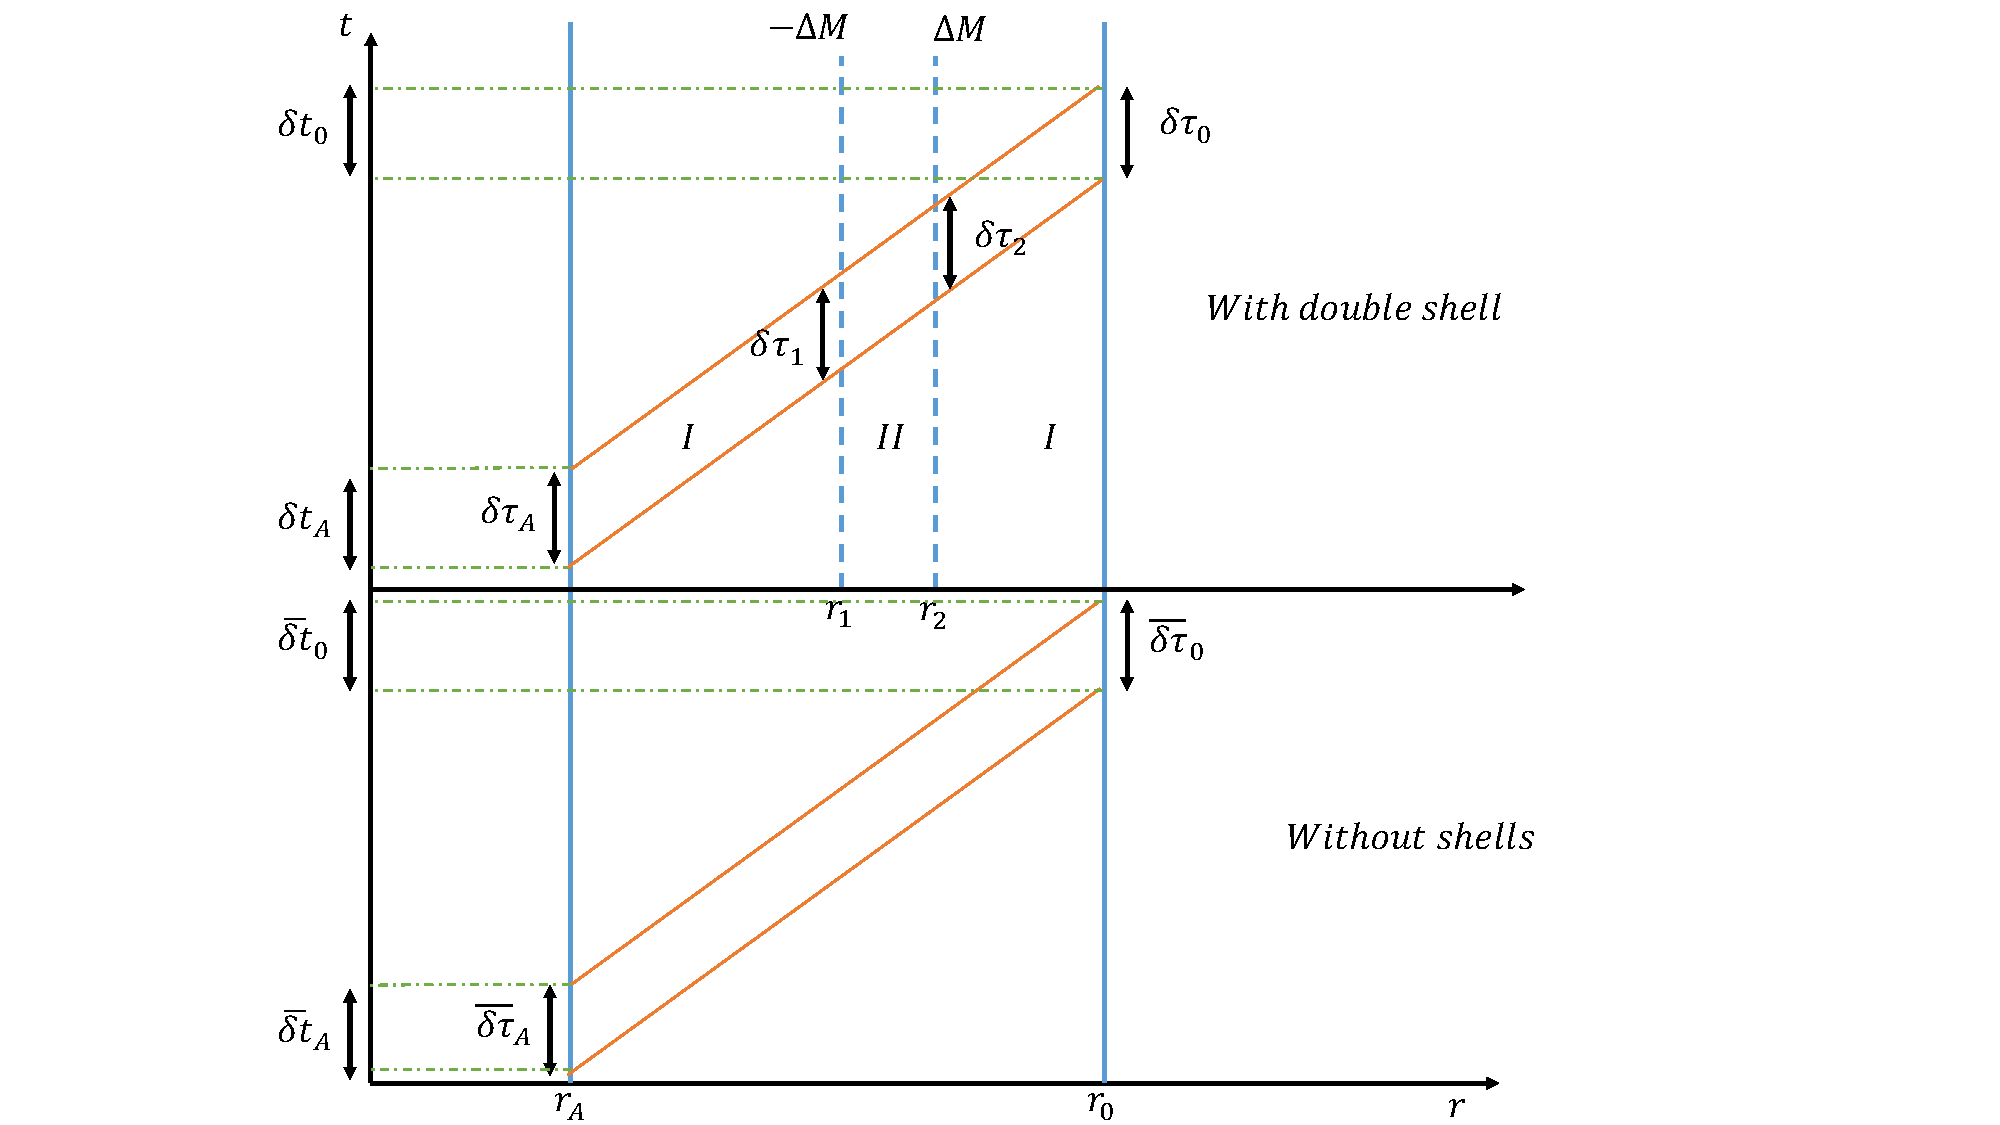
\includegraphics[scale = 0.6]{Propertime.pdf}
\caption{The two parts of this diagrams describe two different scenarios. The trajectories of the photon are the lines in orange. The trajectory of the observer and the position from which the photons are emitted are represented by solid blue lines. The bottom part is a general case of two Hawking photons coming from a distance $r_A$ from the black hole of mass $M$ and arriving at an observer who is at a distance of $r_0$. The top part shows two Hawking photons coming from the same distance $r_A$ from a black hole of mass $M$. Instead of the photons freely propagating through to an observer at $r_0$, they have to cross two shells, represented by blue dotted line, of equal and opposite mass $-\Delta M, \Delta M$ at $r_{1}, r_{2}$ respectively. The regions $I$ represent a metric with mass $M$ and region $II$ represents a metric with mass $M-\Delta M$.}
\label{fig:1}
\end{center}
\end{figure}


In this section we consider the top part of figure \ref{fig:1}. To distinguish the results from the previous section without shell we will not have an overbar in any of the quantities described in this scenario. The same initial conditions for the two Hawking photons are assumed. Using the argument described in the previous section we expect the coordinate time intervals between $r_A$ and $r_1$ to be equal, $\delta t_A = \delta t_1$. Analogously for the coordinate time interval between $r_2$ and $r_0$, $\delta t_2 = \delta t_0$. The new region is between $r_2$ and $r_1$ where the metric is different; it is defined by a mass $M - \Delta M$. The coordinate time interval at $r_1$ will also have a representation in the $II$ metric. Quantities evaluated in the $II$ metric will be denoted by a hat on top. By imposing the physical condition that there cannot be any discontinuities in spacetime we know that the proper times in both the metrics must be the same at $r_1$, $\delta \tau_1 = \delta \hat{\tau}_1$ and this gives a relation between the coordinate time intervals

\begin{equation}
	\delta t_1 = \left( \frac{1 - \frac{ 2(\Delta M -M)}{r_1})}{1 - \frac{ 2M}{r_1}}  \right)^\frac{1}{2} \delta \hat{t}_1.	\label{shell1}
\end{equation}

Applying the same condition to the proper times at $r_2$ gives the analogous relation between the coordinate time intervals at $r_2$, 

\begin{equation}
	\delta t_2 = \left( \frac{1 - \frac{ 2(\Delta M -M)}{r_2})}{1 - \frac{ 2M}{r_2}}  \right)^\frac{1}{2} \delta \hat{t}_2. 	\label{shell2}
\end{equation}

Since $\delta \hat{t}_1$ and $\delta \hat{t}_2$ are both evaluated in the same metric they must be equal and therefore we can combine Eq (\ref{shell1}) and Eq (\ref{shell2}) to give a relation between $\delta t_1$ and $\delta t_2$, 

\begin{eqnarray}
	\delta t_{1} & = & \left( \frac{ \left( 1 - \frac{2 M - \Delta M}{r_{1}} \right) \left( \frac{1 - 2M}{r_{2}} \right)}{\left( 1 - \frac{2M}{r_{1}} \right)  \left( 1 - \frac{2(M - \Delta M)}{r_{2}} \right)} \right)^\frac{1}{2} \delta t_{2}	\nonumber	\\
	& = & \left( \frac{2M - r_2}{2M - r_1} \right)^\frac{1}{2} \left( \frac{ 2(\Delta M - M) + r_1}{2(\Delta M - M) + r_2} \right)^\frac{1}{2} \delta {t}_{2}.
\end{eqnarray}

We see that $\delta t_1 = \delta t_2$ in the limit that $r_1 = r_2$ as then the shells will cancel out their masses and we are left with just metric $I$. By continuing these trajectories forward to the observer at $r_0$ we know that $\delta t_0 = \delta t_2 \approx \delta \tau_0$. 

%\begin{SCfigure}
% \centering
%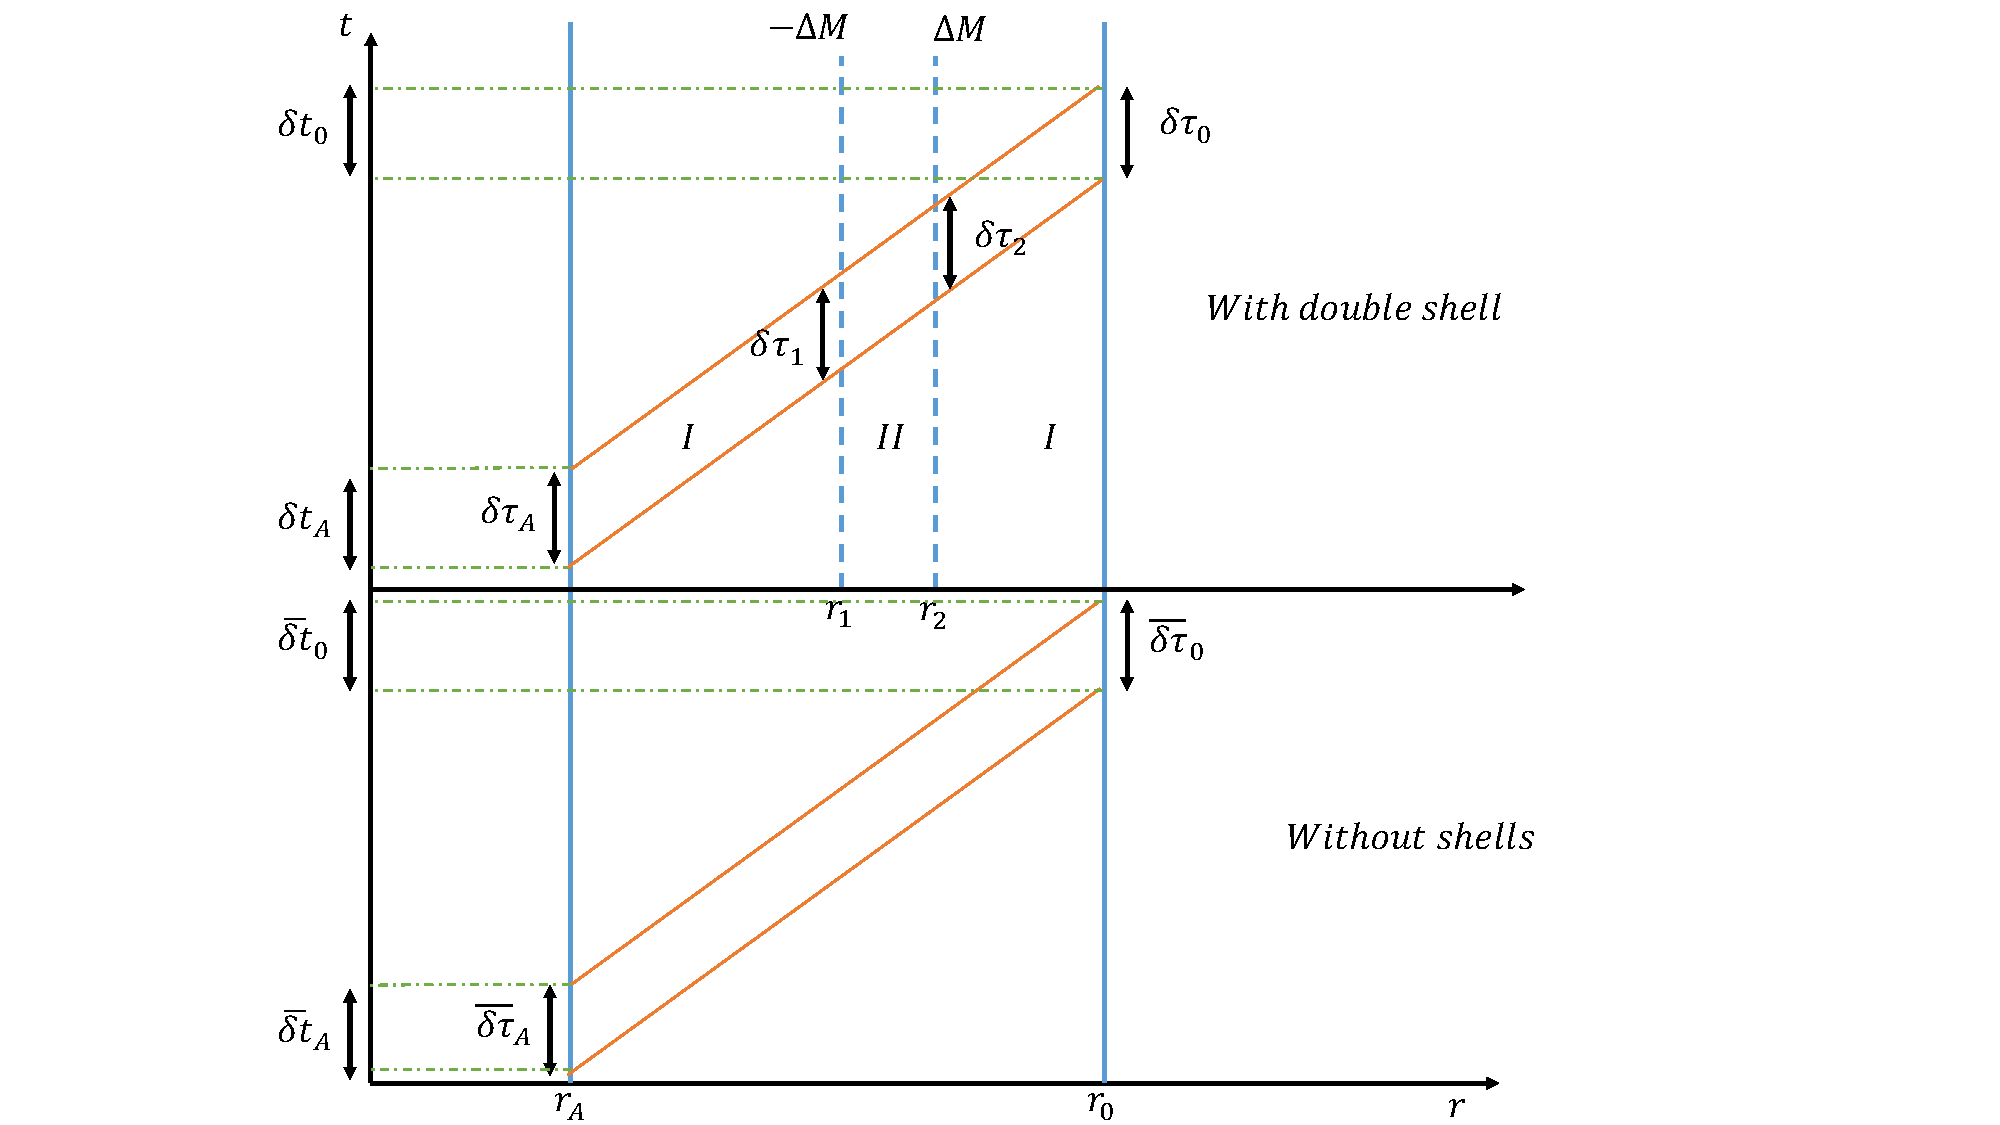
\includegraphics[height= 7 cm]{Propertime.pdf}	\label{fig:1}
%  \caption{The two parts of this diagrams describe two different scenarios. The trajectories of the photon are the lines in orange. The trajectory of the observer and the position from which the photons are emitted are represented by solid blue lines. The bottom part is a general case of two Hawking photons coming from a distance $r_A$ from the black hole of mass $M$ and arriving at an observer who is at a distance of $r_0$. The top part shows two Hawking photons coming from the same distance $r_A$ from a black hole of mass $M$. Instead of the photons freely propagating through to an observer at $r_0$, they have to cross two shells, represented by blue dotted line, of equal and opposite mass $-\Delta M, \Delta M$ at $r_{1}, r_{2}$ respectively. The regions $I$ represent a metric with mass $M$ and region $II$ represents a metric with mass $M-\Delta M$.}
%\end{SCfigure}

%\twocolumngrid

Without shells we saw that the proper time interval $\bar{\delta \tau}_0 \approx \delta t_A$, thus the difference in the proper time intervals with the shells is

\begin{equation}
	\delta \tau_0 - \bar{\delta \tau_0} = \delta t_A \left( \left( \frac{2M - r_2}{2M - r_1} \right)^\frac{1}{2} \left( \frac{ 2(\Delta M - M) + r_1}{2(\Delta M - M) + r_2} \right)^\frac{1}{2} - 1 \right). 	\label{PTD}
\end{equation}
As a check we see that when $r_1 = r_2$, $\delta \tau_0 = \bar{\delta \tau}_0$ as expected. 

We can explore this relation further by going to a region close to the horizon. If we choose $r_1 = 2M + \epsilon_1$ and $r_2 = 2M + \epsilon_2$ where $\epsilon_{1,2} <<1$, the expression in Eq (\ref{PTD}) reduces to 

\begin{equation}
	\delta \tau_0 - \bar{\delta \tau_0} = \left( \left( \frac{\epsilon_2}{\epsilon_1} \left( \frac{2\Delta M + \epsilon_1}{2 \Delta M + \epsilon_2}\right) \right)^\frac{1}{2} - 1 \right) 
\end{equation}

\subsection{Frequency of Hawking photons}

\begin{figure}[h!]
\begin{center}
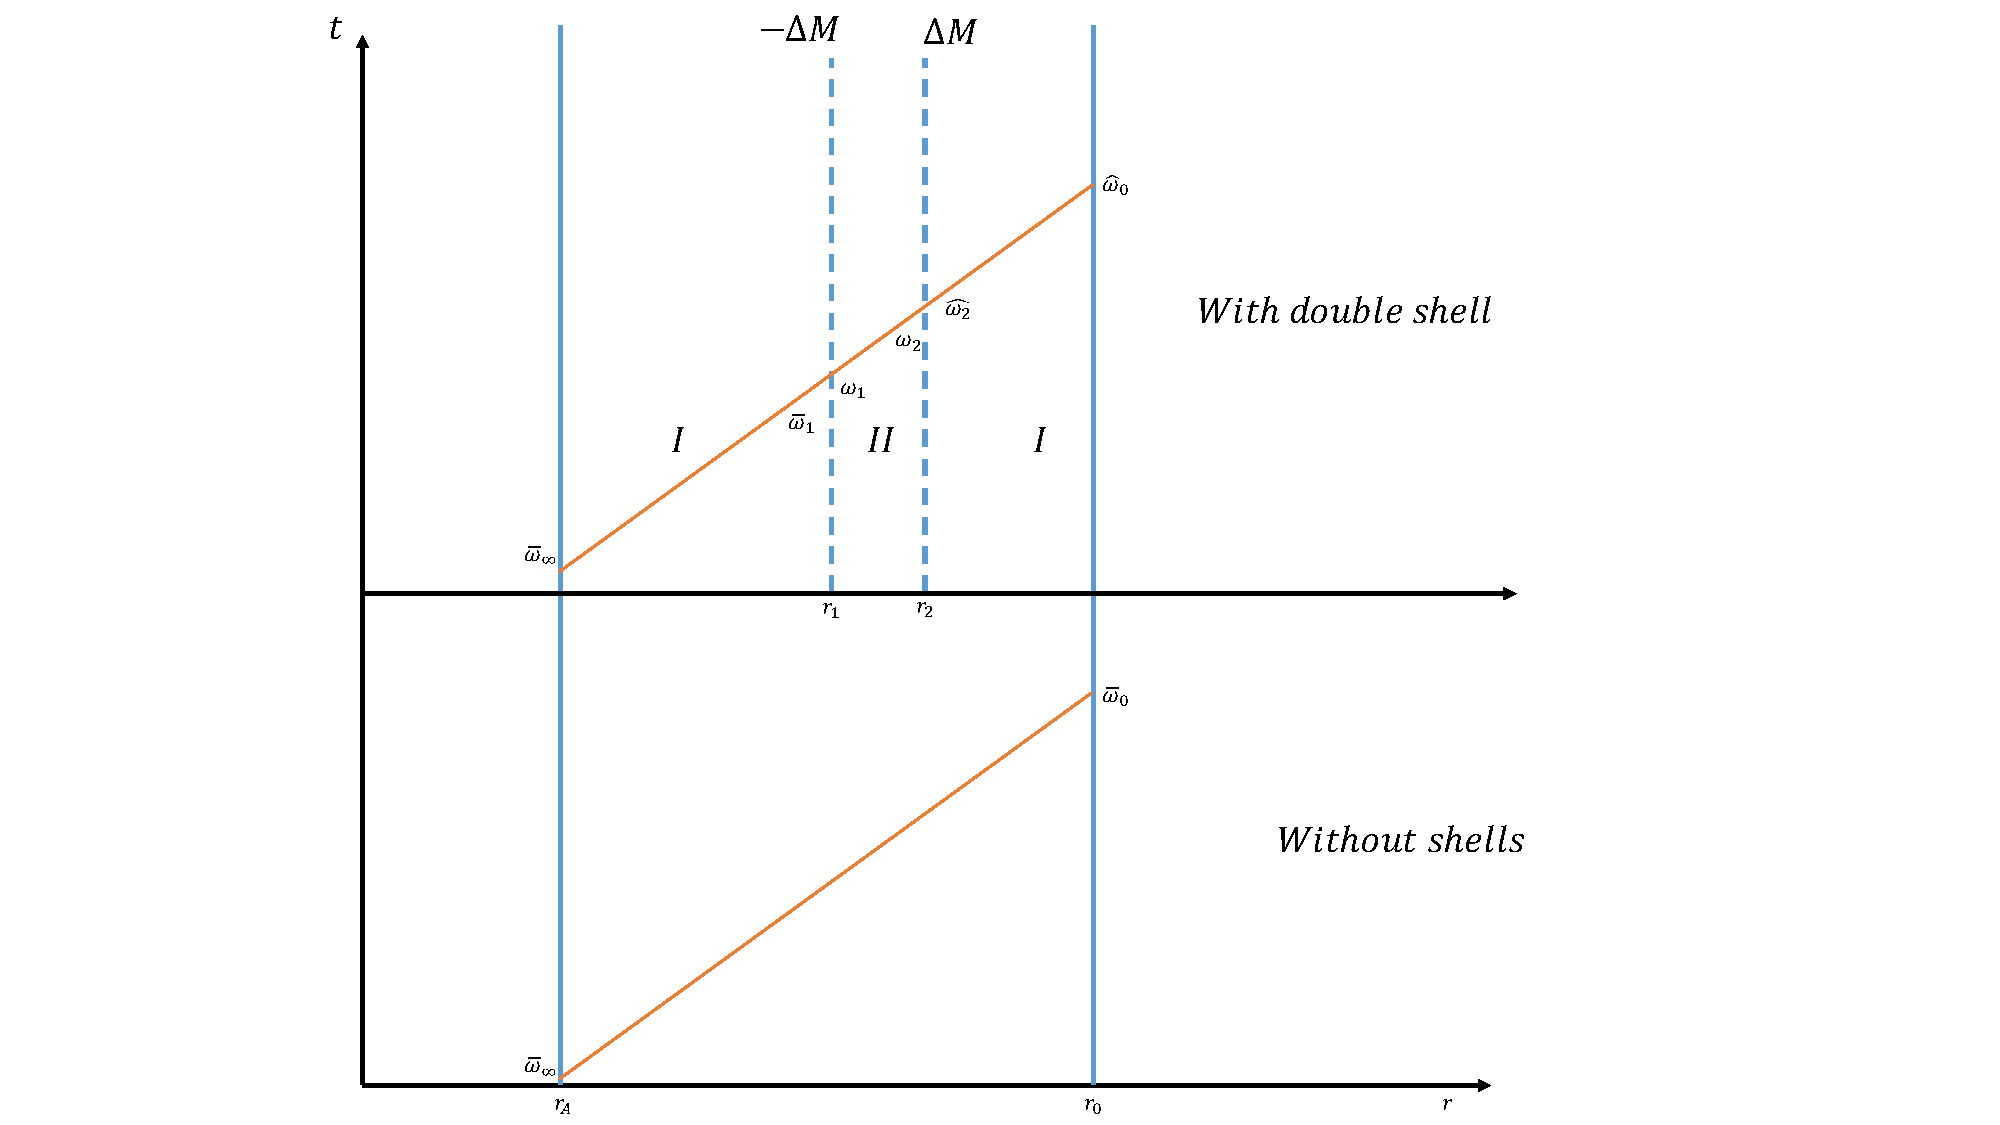
\includegraphics[scale = 0.6]{frequency.pdf}
\caption{This diagram follows the same notation as figure \ref{fig:1} except we are looking at one photon represented by the orange line. The frequency at each relevant point is denoted on the diagram. The quantities in the metric $I$ on the left of the shells are denoted with overbars. Quantities in metric $II$ are denoted without any overbars or hats. Quantities in metric $I$ to the right are denoted with hats on top.}
\label{fig:2}
\end{center}
\end{figure}


\subsubsection{Background spacetime}
We can do an analogous calculation to see this effect. Instead of looking at the proper time interval between photons we can consider the shift in frequency of single Hawking photon in the same two scenarios as were described in the previous section. We can write the photon four vector at distance $r$ as

\begin{equation}
	\bar{k}^\mu (\bar{\omega}_\infty, \bar{r}) = \bar{\omega}_\infty \left( \left( 1 - \frac{2M}{\bar{r}_A} \right)^{-1}, \sqrt{ 1 - \frac{\bar{b}^2}{\bar{r}_A^2} \left( 1 - \frac{2M}{\bar{r}_A} \right)}, \frac{\bar{b}}{\bar{r}_A^2}, 0 \right),
\end{equation}
where $\bar{\omega}_\infty$ is the frequency observed by a stationary observer at infinity and $b$ is the impact parameter of the photon. The general four velocity, $\bar{u}^\mu(\bar{r})$ of a stationary object in this geometry is

\begin{equation}
	\bar{u}^\mu(\bar{r}) = \left( \left( 1 - \frac{2M}{\bar{r}} \right)^{-\frac{1}{2}}, 0, 0, 0 \right).
\end{equation}

In the case where there are no shells, $\bar{\omega}_\infty$ is exactly the frequency observed by the observer at $\bar{r}_0$ in the limit that $\bar{r}_0 \rightrrow \infty$. In general, the frequency observed at $\bar{r}_0$, $\bar{\omega}_0$, will be redshifted

\begin{eqnarray}
	\bar{\omega}_0 & = & \bar{k}^\mu(\bar{\omega}_\infty, \bar{r}_0) \bar{u}^\nu(\bar{r}_0) \bar{g}_{\mu \nu}(\bar{r}_0) 	\nonumber	\\
	& = & - \bar{\omega}_\infty \left( 1 - \frac{2M}{\bar{r}_0} \right)^{-\frac{1}{2} }
\end{eqnarray}

of course in the limit $\bar{r}_0 \rightarrow \infty$ we get $\bar{\omega}_0 = -\bar{\omega}_\infty$. 

\subsubsection{Introducing perturbations: Double shells}

The frequency measured at $r_1$ in metric $I$, $\bar{\omega}_1$ is 

\begin{equation}
	\bar{\omega}_1 = - \bar{\omega}_\infty \left (1 - \frac{2M}{\bar{r}_1} \right)^{-\frac{1}{2}}.
\end{equation}

In metric $II$ the observed frequency $\omega_1$ is 

\begin{eqnarray}
	\omega_1 & = & g_{\mu \nu}(r_1) k^\mu(\omega_\infty, r_1) u^\nu(r_1)	\nonumber	\\
	& = & - \omega_\infty \left( 1 - \frac{2(M- \Delta M)}{r_1} \right)^{-\frac{1}{2}}.
\end{eqnarray}

Since $\omega_1$ is a physical quantity we expect it to be the same in both in metrics, $\omega_1 = \bar{\omega}_1$ and also we expect $r_1 = \bar{r}_1, r_2 = \bar{r}_2$ (since the radius of the shell corresponds to a physical sphere of radius of $r$). This gives a relation between $\omega_\infty$ and $\bar{\omega}_\infty$

\begin{equation}
	\bar{\omega}_\infty = \omega_\infty \left( 1 - \frac{2 \Delta M}{2(\Delta M  - M)+ r_1} \right)^\frac{1}{2}.	\label{13}
\end{equation}

At $r_2$ we can again equate the observed frequencies in both metrics. In this case we define the frequency observed at infinity in metric $I$ on the right side of $r_2$ as $\hat{\omega}_\infty$, i.e the photon vector in metric $I$ for $r > r_2$ is $\hat{k}$ (But we expect the four velocity of the shell to be $\bar{u}_2$). From $k^\mu(\omega_2, r_2) u^\nu(r_2) g_{\mu \nu}(r_2) = \hat{k}^\mu(\bar{r}_2) \bar{u}^\nu(\bar{r}_2) \bar{g}_{\mu \nu} (\bar{r}_2)$ we have

\begin{equation}
	\hat{\omega}_\infty = \omega_\infty \left( 1 - \frac{2 \Delta M}{2(M-\Delta M) + r_2} \right)^\frac{1}{2}.	\label{14}
\end{equation}

By combining Eq (\ref{13}) and (\ref{14}) we get 

\begin{equation}
	\hat{\omega}_\infty = \bar{\omega}_\infty \left( \frac{(2 (\Delta M - M) + r_1)(r_2 - 2M)}{(r_1 - 2M)(2(\Delta M - M) + r_2)} \right)^\frac{1}{2}
\end{equation}

The observed frequency at $r_0$, $\hat{\omega}_0$, is

\begin{eqnarray}
	\hat{\omega}_0 & = & u^\mu(r_0) k^\nu(\hat{\omega}_\infty, r_0) g_{\mu \nu}(r_0) 	\nonumber	\\
	& = & - \bar{\omega}_\infty \left( 1 - \frac{2M}{r_0} \right)^{-\frac{1}{2}}  \left( \frac{(2 (\Delta M - M) + r_1)(r_2 - 2M)}{(r_1 - 2M)(2(\Delta M - M) + r_2)} \right)^\frac{1}{2}
\end{eqnarray}

In the limit that $r_0 \rightarrow \infty$, 

\begin{equation}
	\hat{\omega}_0 = - \bar{\omega}_\infty \left( \frac{(2 (\Delta M - M) + r_1)(r_2 - 2M)}{(r_1 - 2M)(2(\Delta M - M) + r_2)} \right)^\frac{1}{2}
\end{equation}

Looking at dynamics close to the horizon, 

\begin{eqnarray}
	r_1 & = & 2M + \epsilon_1	\nonumber	\\
	r_2 & = & 2M + \epsilon_2
\end{eqnarray}

we get

\begin{equation}
	\hat{\omega}_0 = - \bar{\omega}_\infty \left( \frac{\epsilon_2}{\epsilon_1} \left( \frac{2 \Delta M + \epsilon_1}{2 \Delta M + \epsilon_2} \right) \right)^\frac{1}{2}
\end{equation}
















\bibliography{all_active}


\end{document}